\newpage


\section{Existujúce riešenia}

Existuje veľké množstvo riešení problému s dynamickým odporúčaním. Všetky pracujú s nejakou množinou vlastností, tém alebo kľúčových slov, ku ktorým sa snažia vypočítať pravdepodobnosť, že práve daná téma, kľúčové slovo alebo vlastnosť je pre používateľa najzaujímavejšia a následne mu odporučiť vyhľadávané subjekty, z danou vlastnosťou.

Postup riešenia sa dá rozdeliť na niekoľko podproblémov, ktoré sa dajú riešiť osobitne:

\begin{itemize}
\item{získavanie vlastnosti dokumentov,}
\item{získavanie používateľskej spätnej väzby,}
\item{ukladanie používateľského profilu,}
\item{porovnávanie používateľových preferencií s dokumentami,}
\item{starnutie preferencií,}
\item{triedenie preferencií na krátkodobé a dlhodobé,}
\end{itemize}

\subsection{Kategorizácia dokumentov}

Aby sme mohli odporučiť dokument, musíme získať nejaké jeho vlastnosti, ktoré budeme vedieť priradiť k používateľskému profilu. 

\paragraph{Kategorizovanie na základe typu dokumentu}

Prvou skupinou vlastností určujúcich dokument je jeho typ. Dokumenty môžu byť piatich typov, pričom sú možné aj rôzne kombinácie typov, teda môže nastať, že mám text s akordmi pričom sólo daného hudobného diela je zapísané pomocou tabov. Takže pre každý dokument \(d_j\) z množiny dokumentov \(D = (d_0, d_1, \cdots, d_n)\) budem mať určené štyri premenné \(d_j = (a_j, x_j, p_j, t_j, n_j)\), ktoré budú nadobúdať buď hodnotu \(1\) alebo \(0\) na základe toho, či dokument patrí do danej kategórie alebo nie. Jednotlivé premenné reprezentujú nasledovné druhy obsahu:

\begin{itemize}
\item{\(a_j\) určuje či dokument \(j\) obsahuje akordy,}
\item{\(x_j\) určuje či dokument \(j\) obsahuje text,}
\item{\(p_j\) určuje či dokument \(j\) obsahuje preklad textu,}
\item{\(t_j\) určuje či dokument \(j\) obsahuje taby,}
\item{\(n_j\) určuje či dokument \(j\) obsahuje noty,}
\end{itemize}

\paragraph{Kategorizovanie na základe hudobnej štruktúry}

Hudobné dokumenty sa dajú ďalej deliť z hľadiska hudobnej štruktúry. Pre dokument \(d_j\) vieme určiť niekoľko časti štruktúry, Jeden hudobný dokument nemusí obsahovať všetky súčasti hudobného diela. Tak isto jedno hudobné dielo nemusí používať všetky štandardné súčasti. V zásade rozoznávame a určujem tieto štandardné časti hudobných diel \cite{1}:

\begin{itemize}
\item{predohra,}
\item{medzihra,}
\item{refrén,}
\item{ukončenie (angl. Outro),}
\item{sólo alebo inštrumentálna časť}\ignore{Nájdi článok,}
\end{itemize}

No toto nie je najmenšie možné delenie, z hľadiska kompozície môžeme ešte hudobné dielo rozdeliť na jednotlive nástroje, ktoré vykonávajú dané prevedenie hudobného diela. Tak isto sa dané časti môžu rozlišovať variáciami motívu\cite{12},

\paragraph{Kategorizovanie na základe prevedenia}

Ďalej môžeme hudobné diela deliť na základe konkrétneho prevedenia. Niektoré hudobné diela môžu mať aj niekoľko prevedení. Prevedenia sa dajú charakterizovať na základe miesta, použitých nástrojov alebo hudobníkov, ktorí dané prevedenie zahrali.

\paragraph{Kategorizovanie na základe žánru}

Žáner je asi jeden z najdôležitejších spôsobov kategorizovania hudobných diel. Hlavnými ukazovateľmi žánru hudobného diela sú akustické vlastnosti zvuku a téma textu. Momentálne existuje veľké množstvo hudobných štýlov a spôsobov zaradenia, avšak chýba určitá štandardizácia. Následkom toho či už automatické určovanie alebo určovanie bežným človekom dosahuje asi presnosť 70\% \cite{5}.Tak isto z hľadiska kompozície, každá časť hudobného diela môže obsahovať iný hudobný žáner\cite{3}.

\subsection{Získavanie používateľskej spätnej väzby}

Aby sme mohli presne určiť či daný hudobný dokument vyhovuje používateľovi, je potrebné nejakým spôsobom získať jeho spätnú väzbu. V zásade existujú dva spôsoby získavania spätnej väzby:

\begin{itemize}
\item{explicitná (používateľ vedome poskytne spätnú väzbu napr. hodnotenie dokumentu),}
\item{implicitná (používateľ o tejto spätnej väzbe nevie, používajú sa agenti ktorí ho monitorujú napr. počítanie času stráveného na stránke),}
\end{itemize}

\paragraph{Identifikácia používateľa}

Prvým krokom pri získavaní spätnej väzby je identifikácia používateľa, najpoužívanejší spôsob identifikácie používateľa je pomocou prihlásenia, kedy používateľ pred použitím systému identifikuje sám seba podľa mena a hesla. Tento spôsob sa radi medzi spôsoby ktoré vyžadujú zásah používateľa. 

Ďalšou alternatívou v tomto smere je softvérový agent, ktorého si používateľ nainštaluje u seba na počítači. Nevýhodou oproti predchádzajúcemu prístupu je že používateľ musí agenta nainštalovať na každom zariadení ktoré používa.

Alternatívy ktoré nevyžadujú používateľov zásah sú pomocou súborov cookie \ignore{Nájdi ako preložiť} a pomocou relácií. Obidve tieto alternatívy trpia tím že ak sa používateľ pristupuje z iného zariadenia nebudú ho vedieť identifikovať\cite{4}.

\subsection{Profil používateľa}

Rozlišujeme niekoľko druhov používateľských profilov, základe delenie je minimálny (angl. core) a rozšírený (angl. extended) profil. Minimálny používateľsky profil obsahuje čisto informácie o používateľových preferenciách, zatiaľ čo rozšírený používateľský profil obsahuje aj demografické informácie (vek, rodná krajina, vzdelanie, schopnosti atď,)\cite{4}

\paragraph{Model profilu používateľa}

Je viacero spôsobov ako uložiť profil používateľa, každý má svoje špecifiká a umožňuje iným spôsobom vykonávať odhadovanie používateľových záujmov.

\paragraph{Profil kľúčových slov(angl. keywords profiles)}

Profil kľúčových slov je matica o dimenziách používatelia x kľúčové slová. Na základe toho aké jednotlivé súradnice matice môžu dosahovať hodnoty 0 ak dané kľúčové slovo patrí do používateľovho profilu a 0 ak nie. Na obrázku 1. môžeme vidieť príklad v ktorom máme používateľa Používateľ 0 ktorý nemá žiadne kľúčové slová, následne Používateľa 1 ktorý používa kľúčové slová 1 a 2 a Používateľa 2 ktorý používa kľúčové slovo 1.

\begin{figure}
    \begin{center}
        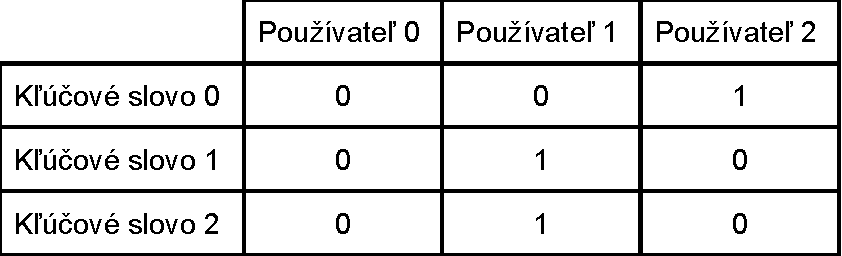
\includegraphics[scale=0.55]{keywordprfile}
        \caption{Ukážka profilu kľúčových slov.}
            \label{Profil klúčovích slov}
    \end{center}
\end{figure}

\paragraph{Profil sémantickej siete (angl. Semantic network profile)}

Tento tip profilu sa používa najmä v systémoch používajúcich rozširovanie používateľských vyhľadávacích reťazcov. Základom tohoto profilu je sémantická sieť ktorej príklad môžeme vidieť na obrázku 2.

\begin{figure}
    \begin{center}
        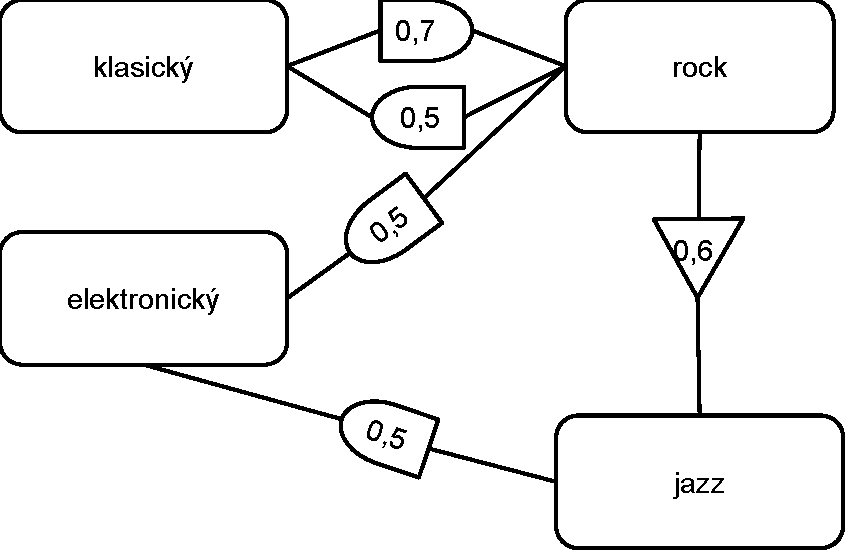
\includegraphics[scale=0.55]{semanticnetwork}
        \caption{Ukážka sémantickej siete}
    \end{center}
\end{figure}

Sémantická sieť je orientovaný graf v ktorom vrcholmi sú preferencie alebo vlastnosti dokumentov, zatiaľ čo hrany sú ich vzťahy. Vzťahy môžu byť niekoľkých typov:

\begin{itemize}
\item{konjunkcia,}
\item{disjunkcia,}
\item{substitúcia,}
\item{negácia,}
\end{itemize}

\subsection{Starnutie profilu}

Keďže používateľové zaujmi sú dynamické a menia sa v čase, môžeme implementovať niekoľko modelov starnutia preferencií.

\paragraph{Polia-urn model\ignore{prelož}}

Mám množinu záujmov \(D = (d_0, d_1, \cdots d_n)\), pre každý záujem \(d_j\) ukladám počet vybratí daného záujmu \(s_j\). Pravdepodobnosť znovu vybratia záujmu dostanem pomocou:

\[\frac{s_j}{\sum\limits_{i=1}^n s_i}\]

Kde n je rovné počtu záujmov. Tento model nezávisí od poradia v akom boli prejavené zaujmi.

Pravdepodobnosť že dosiahnem určitú kombináciu \(S = (s_0, s_1, \cdots ,s_n)\) je vyjadrená pomocou:

\[\frac{1}{\sum\limits_{i=1}^n s_i}\]

\cite{6}

\paragraph{Polčas rozpadu}

Jednou z možností ako zabezpečiť starnutie používateľského profilu je využiť funkciu exponenciálneho polčasu rozpadu. Táto funkcia sa hlavne využíva pri datovaní veku uhlíka, avšak dá sa použiť aj ako funkcia starnutia používateľových preferencií. Základom tohoto prístupu je následujúci vzorec:

\[N(t) = N_0e^{-k/t}\]

Aby sme mohli tento algoritmus použiť, musíme si určiť polčas rozpadu preferencie. Následne si na základe polčasu rozpadu vypočítam parameter \(k\), Ten sa dá po odvodení určiť z následujúceho vzorca.

\[k = \frac{\ln{\frac{1}{2}}}{t_r}\]\cite{7}

Kde \(t_r\) je polčas rozpadu. Tento model umožňuje vytvorenie viacerých rýchlosti starnutia pre krátkodobe a dlhodobé záujmy\cite{8}.


\subsection{Geometrické porovnávanie vlastnosti dokumentov z preferenciami}

Pri tomto spôsobe sa relevancia dokumentu \(d_i\) pre používateľa \(u_j\) bude určovať premietnutím dokumentu do priestoru ako vektor \(d_j=(p_0, p_1\cdots p_n)\) kde \(p_0, \cdots p_n\) sú vlastnosti dokumentu, následne sa do toho istého priestoru premietne aj používateľ, pričom dimenzie budú preferencie používateľa \(u_i=(p_0, p_1 \cdots p_n)\). Podobnosť týchto vektorov sa následne vyhodnotí pomocou nasledujúceho vzorca:

\[cos \theta = \frac{d_j * q}{||d_j||*||q||}\]



Pričom \(||d_j||\) a \(||q||\) sú normalizované vektory\cite{9}.


\subsection{Kolaboratívne filtrovanie}

Kolaboratívne filtrovanie je postup pri ktorom odporúčam používateľovi na základe podobnosti z iným používateľom. Kolaboratívne filtrovanie sa delí na založené na obsahu a kolaboratívne filtrovanie  \cite{10}.

Odporúčanie založené na obsahu vychádza z dostupných informácií o diele, teda z vlastnosti diela zatiaľ čo kolaboratívne filtrovanie záleží čisto od explicitnej spätnej väzby používateľa pomocou hodnotenia.

Podľa \cite{10} dosahuje kolaboratívne filtrovanie väčšiu dynamiku. Avšak hrozí problém studeného štartu, teda že novo pridaná položka nebude mať žiadne hodnotenie a preto klesne hneď na spodok odporúčaní. Kolaboratívne filtrovanie môžeme ďalej rozdeliť:

\begin{itemize}
\item{kolaboratívne filtrovanie založené na pamäti}
\item{kolaboratívne filtrovanie založené na modeli}
\item{hybridné kolaboratívne filtrovanie \cite{11}}
\end{itemize}

\paragraph{Kolaboratívne filtrovanie založené na pamäti}

Podobnosť medzi používateľmi sa zisťuje na základe hodnotenia dokumentov. Je použitá heuristicka metóda ktorá zisťuje chýbajúce hodnotenia porovnávaním používateľov a následne doplnenie od najpodobnejšieho používateľa.

\paragraph{Kolaboratívne filtrovanie založené na modeli}

Pracuje z modelom ktorí vytvára hodnotenie a súčasne sa učí na existujúcich dátach.

\paragraph{Hybridné kolaboratívne filtrovanie}

Na obídenie nedostatkov algoritmov kolaboratívneho filtrovania, niektoré aplikácie kombinujú tieto dve metódy.

\section{Váhovanie značiek}

\subsection{Frequencia pojmov (angl. Term Frequency(TF))}

Toto je jeden z najjednoduchších a najstarších prístupov k váhovaniu pojmov,
pricníp spočíva v definovaní si vektora \(F = (t_1, t_2, t_i \cdots t_N\).
Kde \(t_i\) je počet výskytov pojmu v danom parametre dokumentu (názov, žáner,
interpret v našom prípade), ktorý následne vynásobíme váhovacím vektorom. \(\alpha\).

\[F=[t_{názov},t_{žáner},t_{interpret}]\]

\[W_{TF}(t_i) = F_{t_i}.\alpha \]

TODO: Doplň

\subsection{Frequencie pojmov, inverzna frequencia dokumentov (angl. Term Frequency, Inverse Document Frequency (TF*IDF))}

Pri tomto prístupe zahrňujeme do váhovania aj to v akom počte dokumentov
sa daný pojem nachádza, ak sa pojem vyskytuje príliš často, znížime jeho váhu.

TODO: Namiesto x vektorový súčin
\[w_{TF*IDF} = \frac{1}{\log{(DF_{t_i})}} x W_{TF}(t_i)\]

\subsection{BM25 váhovanie}

Tento model je jeden zo štatystických modelov. Tu uvedená verzia je 
jeho modifikácia z TODO: long term zdroje:

\[w_{BM25}(t_i) = \log{
    \frac{(r_{t_i} + 0.5)(N - n_{t_i} + 0.5}
        {(n_{t_i} + 0.5)(R - r_{t_i} + 0.5)}}\],
    }

kde \(N\) je počet všetkých dokumentov, \(n_{t_i}\) je počet
dokumentov obsahujúcich pojem \(t_i\), R je počet dokumentov
ktoré používateľ už navštívil a \(r_{t_i}\) je počet dokumentov ktoré
už používateľ navštíciľ obsahujúcich pojem \(t_i\)

\section{Určovanie adekvátnych dokumentov}

\subsection{Párovanie na základe unikátnych pojmov}

\subsection{Párovanie na základe váh}

\subsection{Jazykový model(angl. Language Model)}

\section{Logistická funkcia}

Logisticka funkcia sa často používa ako pravdepodobnostná funkcia. Funkcia má nasledujúci tvar: 

\[f(t; a,m,n,\tau) = a*\frac{1 + me^{-t/\tau}}{1 + ne^{-t/\tau}}\]

Vo väčšine prípadov sa používa špecialny prípad tejto funkcie meno signusoida.
Signusoida ma $a = 1$, $m = 0$, $n = 0$ a $\tau = 1$ čiže:

\[f(t) = \frac{1}{1 + e^{-t}}\]

Graf tejto funkcie má tvar písmena S


\section{Starnutie záujmov profilu}

\subsection{Krátkodobé záujmy}

\subsection{Dlhodobé záujmy}

\subsection{Sezónne záujmy}
